In our system design, two type of datasets are needed. The first is the social media textual data, which is the most vital to this system, called social media dataset. It contains the implication of potential outbreak of diseases or other healthcare-related information, all the prediction will be made based on it. In addition, to evaluate the accuracy of the prediction convincingly, actual records of diseases are needed to serve as benchmark. 
\section{Social media dataset}
\label{sec:Social media dataset}
Researchers have used the Web as sources of  syndromic surveillance for years, including Google Flu Trends (display the statistics of daily query logs related to influenza), Twitter, Facebook \cite{paul2011you}. 
In this project, we choose one certain social media platform to test our algorithm, that is Twitter. More specifically, we focus on tweets expressed in English. These choices based on the characteristics of Twitter:
\begin{itemize}
    \item Providing location: In our design, the posting location of each post is required. And we found that Twitter provides such information. According to research conducted by \cite{greenwood2016social} in 2016, about 1.6 percent of Twitter users opted in Twitter's location-sharing service.
    \item Availability: Most tweets are available for research. According to \cite{serban2019real}, around 95\% of Twitter users opted in sharing their tweets with public, meaning their tweets can be searched and filtered by keywords without their permission.  
    \item Comparability: In our research, we found that most related works used data from Twitter, which means that Twitter dataset can act as a benchmark to evaluate our algorithm.
    \item Timely: According to \cite{serban2019real}, each tweet is received within seconds of their creation.
    \item High user volume: According to \cite{greenwood2016social}, about 21\% of American citizens use Twitter.
\end{itemize} 

\section{Benchmark} 
Centers for Disease Control and Prevention (CDC)\cite{cdc.gov} is a well-known nation's health protection agency recording diseases (such as flu, heart diseases, COVID-2019) and conditions over the US. Data published by CDC are comparably reliable. In this project, we focus on one certain disease, flu. The benchmark used in this project is Fluview \cite{cdc:fluView}, a weekly-update, influenza surveillance report of the U.S. published by CDC. Such report is a collaborative effort between CDC and its many partners in state, local, and territorial health departments, public health and clinical laboratories, vital statistics offices, healthcare providers, clinics, and emergency departments \cite{cdc.gov}. CDC maintains a surveillance network called Influenza-like Illness Surveillance Network (ILINet), which collect information on outpatient visits to health care providers for influenza-like illness \cite{cdc.gov}. We choose CDC's Fluview as our benchmark because of its:
\begin{itemize}
    \item Reliability: ILINet collects data from about 2600 outpatient healthcare providers across the U.S. weekly \cite{cdc.gov}.
    \item Accessibility: All the reports of Influenza-like Illness (ILI) can be accessed by public.
    \item Comparability: The dataset maps the activity of ILI into levels between 1 to 10, which can be used as labels or targets of our training data.
\end{itemize}
\begin{figure}[!htbp]
   \center
   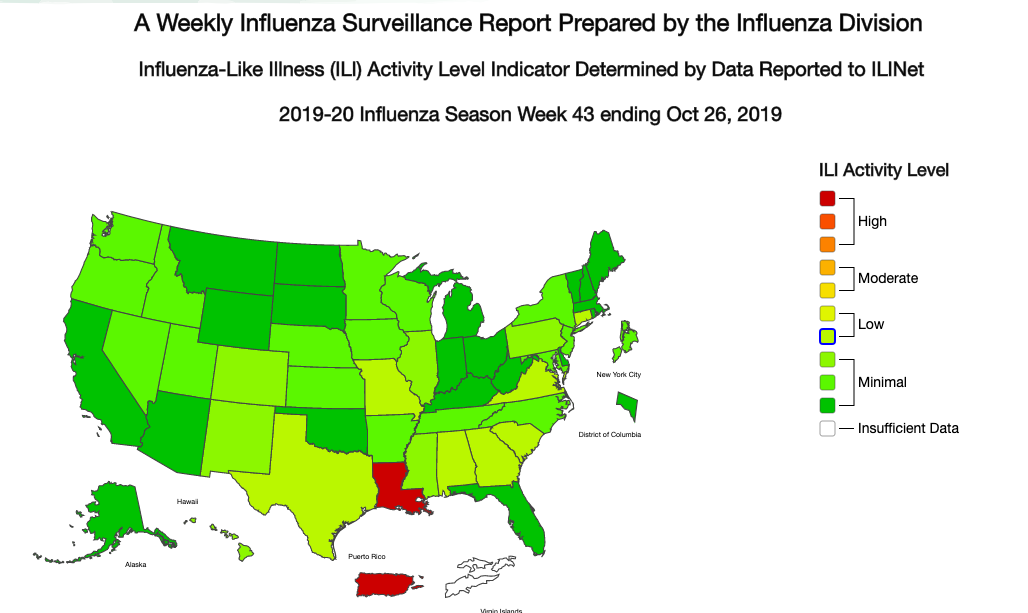
\includegraphics[width=6in]{images/week43.png}
   \caption{Influenza Season Week 43 ending Oct 26, 2019, Source: \href{https://www.cdc.gov/flu/weekly/index.htm\#ILIActivityMap}{Fluview}}
   \label{fig:fluView}
\end{figure}
Figure\ref{fig:fluView} shows the ILI activity levels across the U.S. in Week 43, 2019. It can be seen that the there are 10 levels divided into 3 categories, each level is assigned a unique color.
\section{Data collection}
\label{sec:Data collection}
This section shows the detailed methods of how we collect data and unify the data structure. 
\subsection{Twitter dataset collection}
\label{sec:Twitter dataset}
In this project, we collect Twitter data from Internet Archive\cite{archive}, a non-profit digital library of millions of free books, movies, software, music, websites. It contains daily tweets from Feb 2011 to Jul 2019 (Accessed: Dec 08,2019). All the data are Spritzer version (roughly 1\% of the whole tweets) grabbed from the general twitter stream The number of tweets collected in Oct 05 2018 is 4273031, in Oct 04 2018 is 4337327, in Oct 01 2018 is 4317376, on average is above 4 million per day. All the tweets are stored in json files. Such data volume is sufficient for our research and its data structure is convenient to use. More important, it contains the information we need, which mentioned in section \ref{sec:Social media dataset}. Figure \ref{fig:archive1} shows part of the information those json files contain (geographic and linguistic information are contained but not listed here). In our project, we mainly focus on tweets posted during 2018.\\
\begin{figure}[!htbp]
    \center
    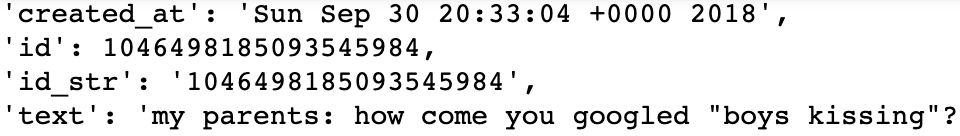
\includegraphics[width=5.5in]{images/archive1.png}
    \caption{Screenshot of Archive's Twitter data}
    \label{fig:archive1}
\end{figure} 

\subsection{Fluview dataset collection}
This data can be downloaded from official websites of Fluview \cite{cdc:fluView} (Accessed: Dec 08,2019), user can customize the data they want to download (the time span of reports). All the information is stored in a single csv file. Figure \ref{fig:fluView1} shows the structure of the data. 
\begin{figure}[!htbp]
    \center
    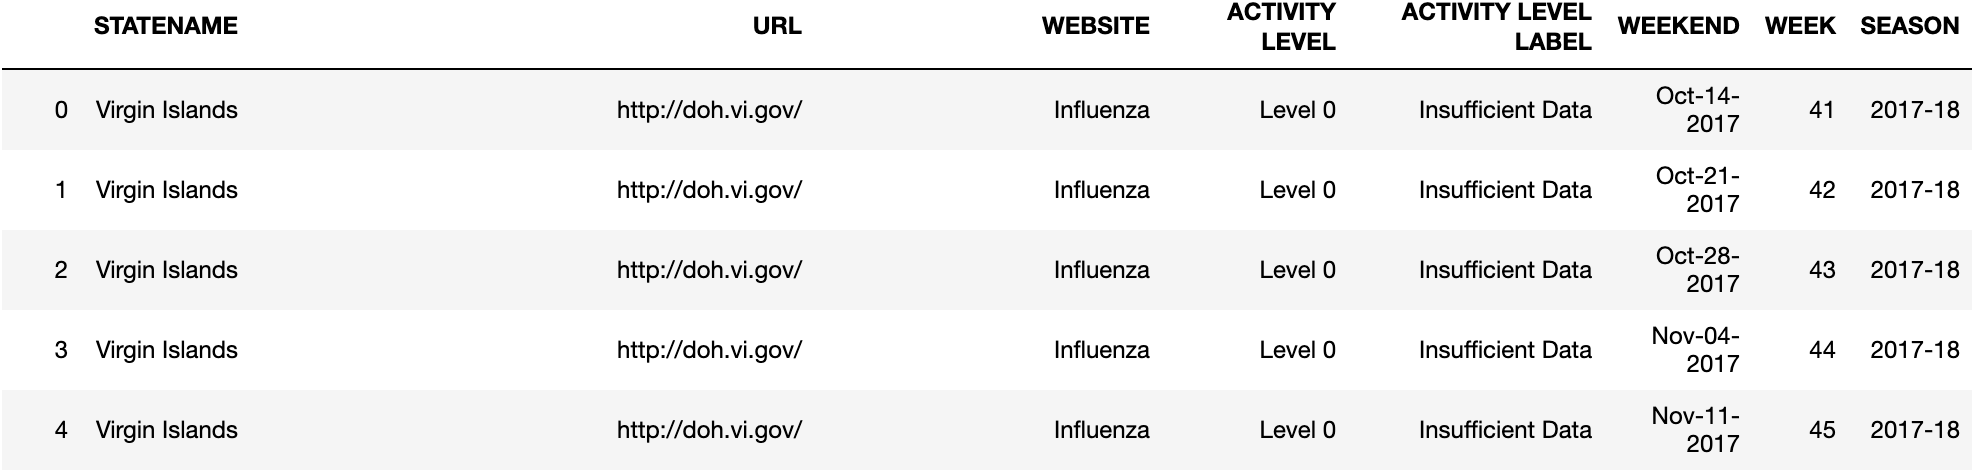
\includegraphics[width=5.5in]{images/fluView1.png}
    \caption{Screenshot of Fluview's report}
    \label{fig:fluView1}
\end{figure}
\\
Our data structure is a cut-down version of it, where ``URL'' and ``WEBSITE'' columns are deleted. ``WEEKEND'' is transformed into the format we used in Twitter dataset.

\section{Data Preprocessing}
\label{sec:Preprocessing}
Data preprocessing is the first stage of a typical text classification framework. According to experiment conducted by \cite{uysal2014impact}, different combination of preprocessing methods can influence the accuracy of prediction. However, there is no best combination for all tasks. Some strategies can improve classification success of certain tasks while lower that of others.
\begin{figure}[!htbp]
    \centering
    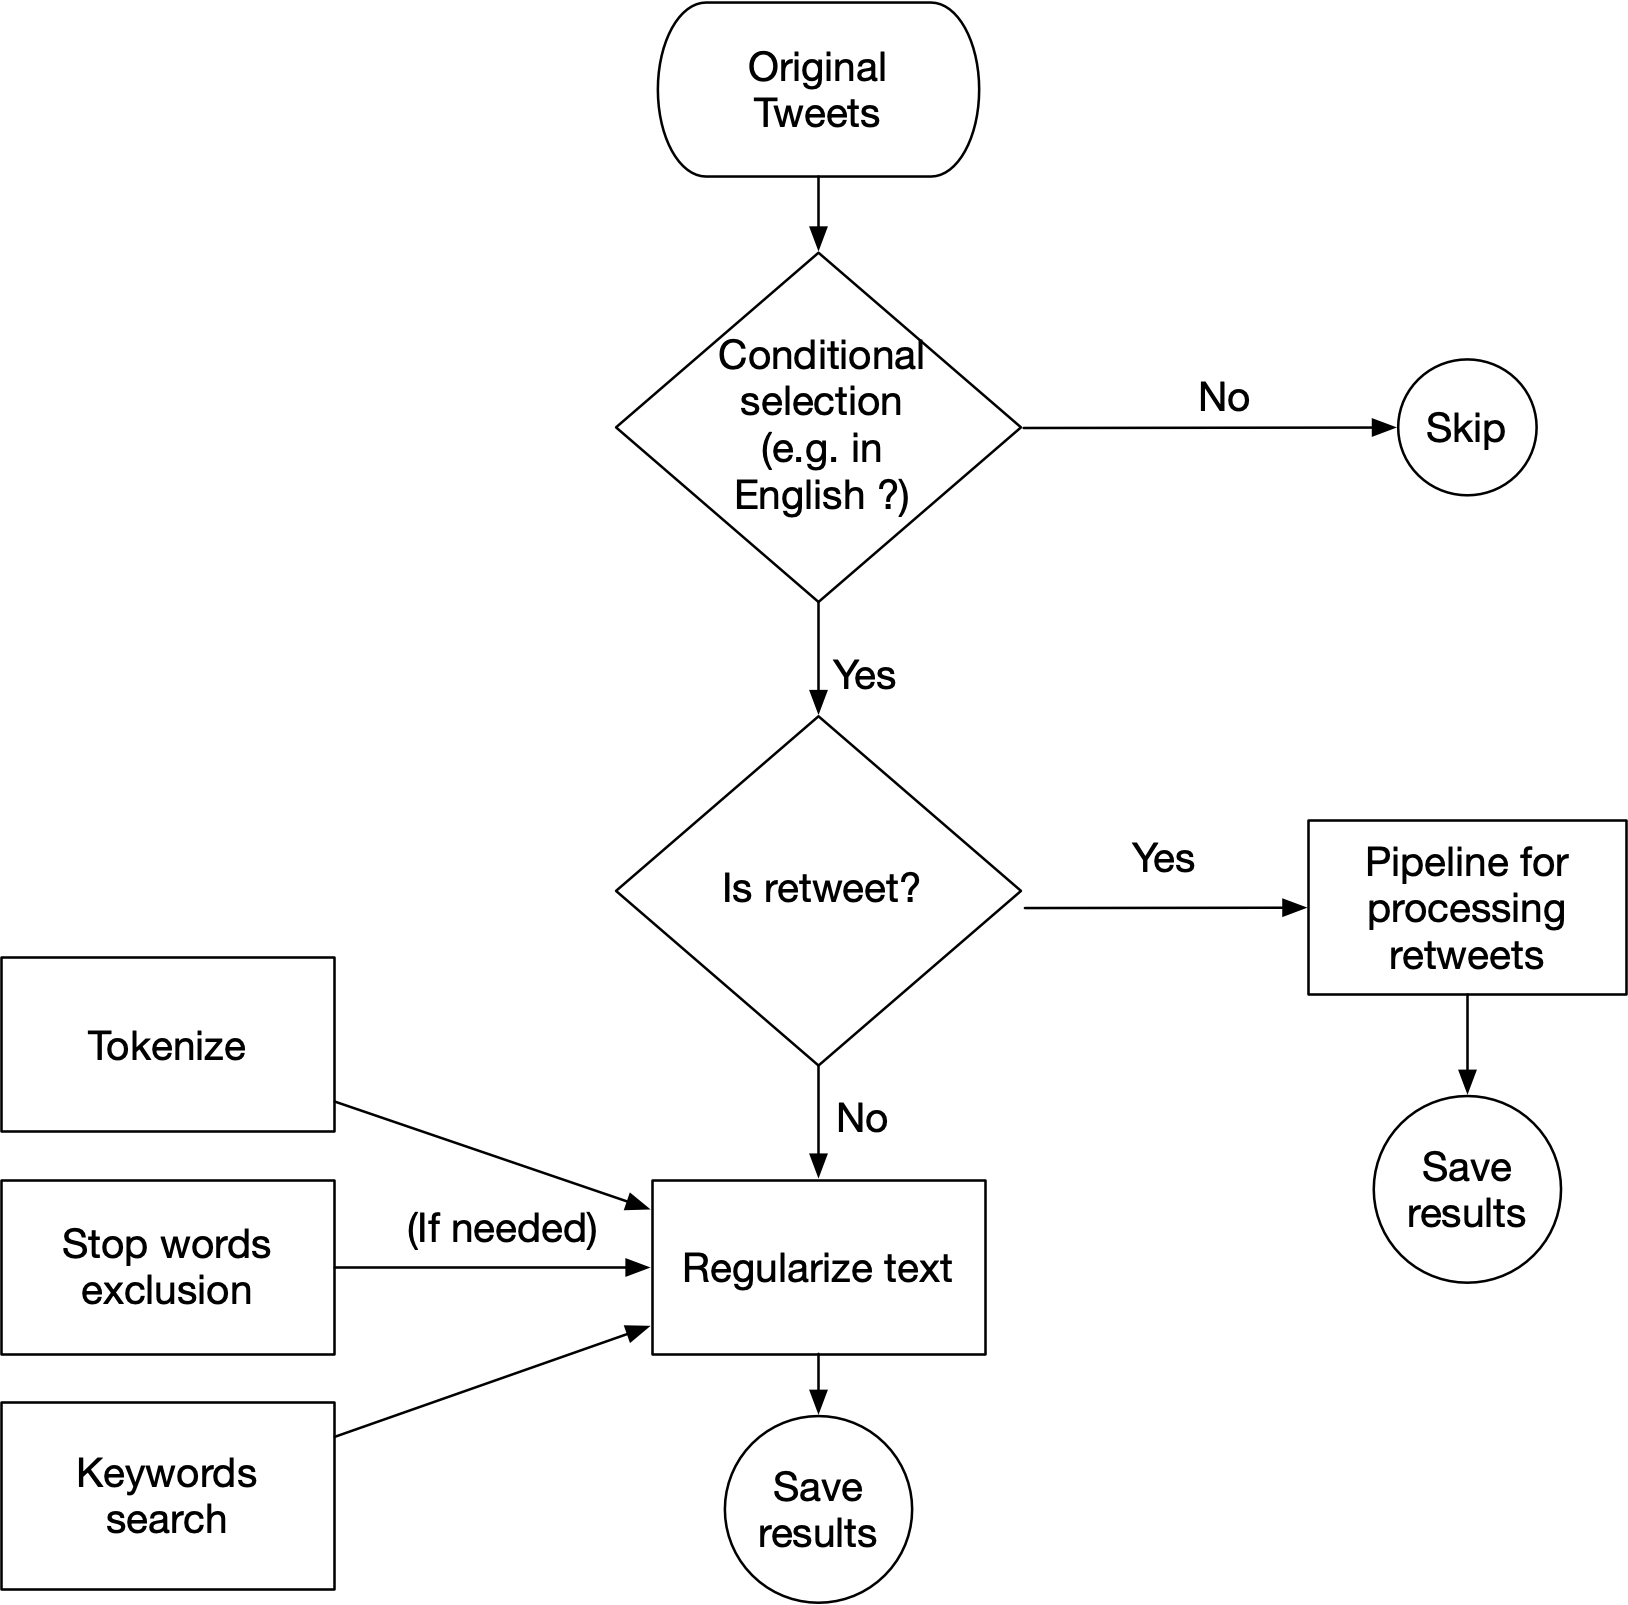
\includegraphics[height=3in]{pipeline.jpg}
    \caption{Common pipeline of text preprocessing}
    \label{fig:pipeline}
\end{figure} 
Figure \ref{fig:pipeline} shows some common steps used in NLP for preprocessing textual data. Following sub-sections explain the details of our preprocessing methods designed for this project.
\subsection{Unify data structure}
\label{sec:Unify data structure}
In section \ref{sec:Data collector design}, we mentioned a unified data structure of our datasets. The aim of this stage is to unify and regularize all the metadata before analysis. \\
\\The Fluview dataset is well structured (see Figure \ref{fig:fluView1}), and can be used in our system directly (we used its ``STATENAME", ``ACTIVITY LEVEL", ``ACTIVITY LEVEL LABEL'' and ``WEEK'' columns). One point should be noticed here is that the STATENAME used in Fluview dataset can be different from that in Twitter (Twitter' users can set their own location), therefore, we created a unified name list of states and a function designed to regularize different geographic information.\\
\\
Our social media dataset's structure is built on Twitter's official data structure \cite{twitter_dev}, and we only reserve the information we may use. It is a hashmap with 5 keys: ``created\_at'', ``text'', ``location'' and ``coordinates'', ``place''. We regularize the time into format Year/Month/Day (2018/10/01) and store it in ``created\_at'' keys, exclude other information (see Figure \ref{fig:social_data_sture}). Note that in the metadata, there are massive ``deleted'' tweets, which contain no textual information, and we removed all such data.
\begin{figure}[!bp]
    \centering
    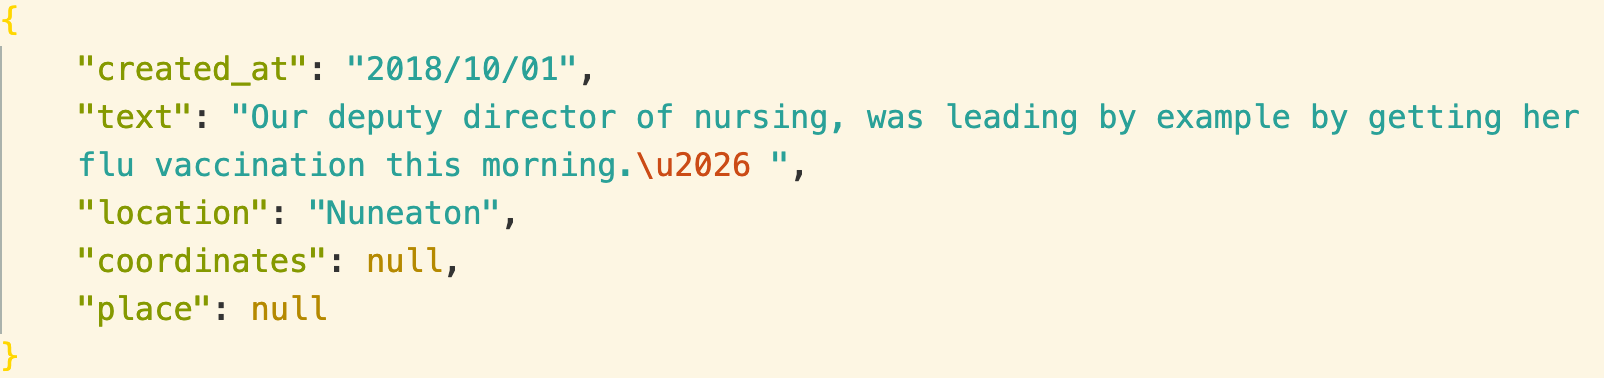
\includegraphics[width=5in]{images/dataset1.png}
    \caption{Screenshot of unified structure of social media dataset}
    \label{fig:social_data_sture}
\end{figure}
According twitter's official document \cite{twitter_dev}, there are two classes of geographical metadata in Tweet data: (1) Tweet location, which is available when users share location at time of Tweet; (2) Account Location: a free-form character field set in user's profile and may or may not contain metadata that can be geo-referenced. ``location'' attribute stores the user-defined placename. ``coordinates'' attribute provides the exact location of a tweet (in long-lat order) but has no placename and only available when the location is assigned. ``place'' attribute is always present when a Tweet is geo-tagged, and it contains Twitter ``place'' with a display name and type. Here we keep all these three keys, and ``place'' key gets the first priority when we extract location of tweet. Figure \ref{fig:twitter_place} shows a sample of Twitter ``place''. Note that most data don't contain ``location'', ``coordinates'' and ``place'' keys, which is expected in section \ref{sec:Social media dataset}.
\begin{figure}[!htbp]
    \centering
    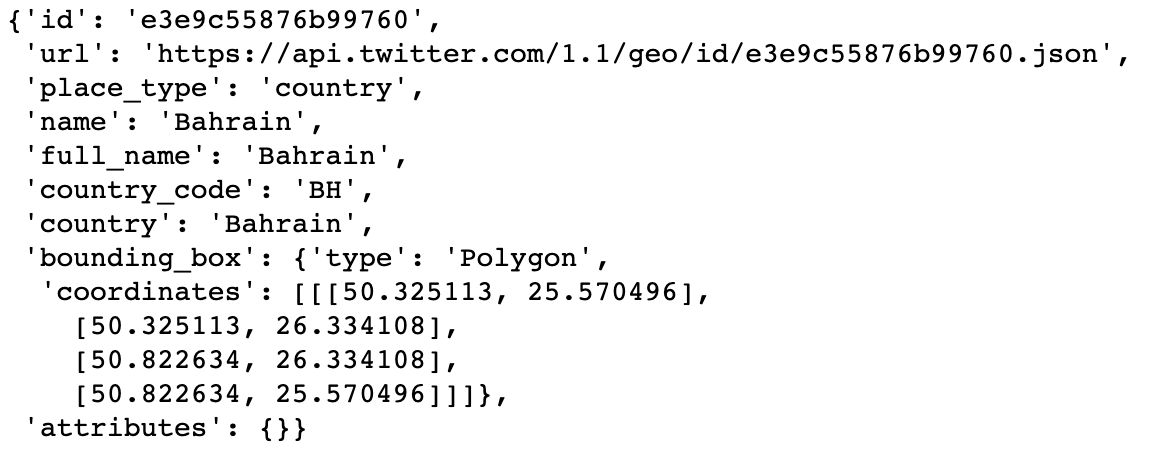
\includegraphics[width=5in]{images/twitter_place.png}
    \caption{Screenshot of Twitter's place object from our dataset}
    \label{fig:twitter_place}
\end{figure}

\subsection{Text regularization}
As mentioned in our design (\ref{sec:Data preprocessor design}), the original text is unstructured, which can not be put in to our model directly and hard for labeling. In addition, each dataset has its own structure, meaning that there is no common regularization rule can be applied to all tasks. Here our regularization rule is built on the observation of our dataset and on our judgement. Followings are common formats we observed and removed (or modified) in our dataset, expressed in regular expression (Python version):
    \begin{itemize}
        \item retweet: retweeting is a way of forwarding content to others (like forwarding an email). It starts with a ``RT \@'' pattern. As we mentioned in section \ref{sec:Manually screening}, we removed all retweets.
        \item @ and \# Tags: in social media, @ refers to a person/group in a conversation, and the \# refers to a topic of conversation. Their regular expression are ``\@+[\verb|\|S]*'' and ``\#+[\verb|\|S]*'' respectively. In our preliminary filtered dataset, we found that some topics contain words in our inclusion list, such as \#ALDUBFever4ever. We exclude them. 
        \item URL links: some tweets contain URL links starting with ``http'', ``ftp'' or ``https'', which can't contribute to our classification. Its regular expression is:\\``http[s]?://(?:[a-zA-Z]$|$[0-9]$|$[\$-\_@.\&+]$|$[!*\verb|\|(\verb|\|),]$|$(?:\%[0-9a-fA-F][0-9a-fA-F]))+''
        \item emoji: emojis in our dataset are encoded in unicode, inspired by \cite{serban2019real}, some of them can be translated into their name based on emoticon dictionaries. Through our search, we find a Python library called \href{https://pypi.org/project/emoji/} {emoji(version 0.5.4}), which embedded the full emoji list from \cite{emo_list} and can help us to translate emoji into text through function call \cite{pytho_emo}. Figue \ref{fig:emo_lib} shows a example how to use this library, the translated emojis are embraced by `:' signs by default. In our implementation, each translated emoji is assigned a prefix `emo\_' to identify it, and we separate emojis with a blank space for split convenience.
        \begin{figure}[!htbp]
            \centering
            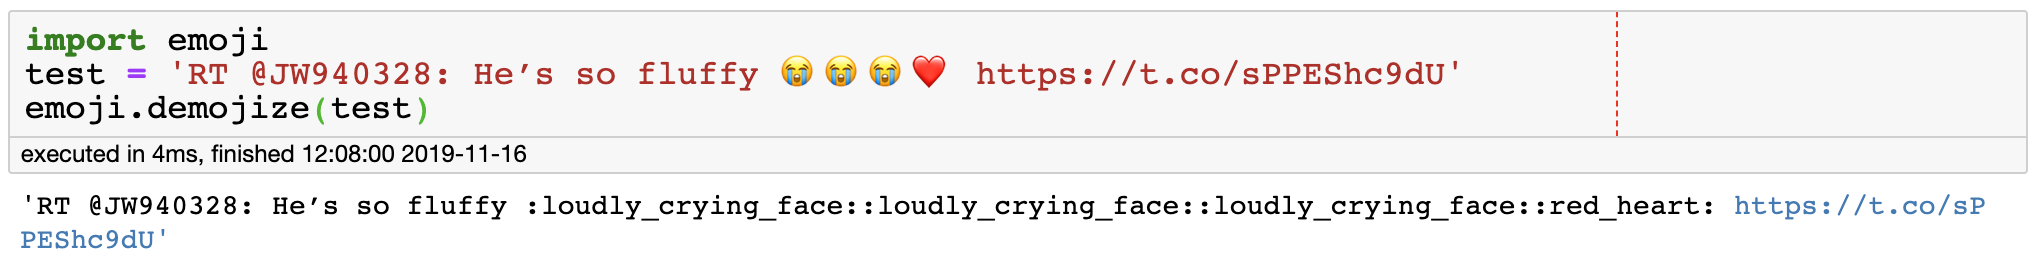
\includegraphics[width=5in]{images/emoji_lib.png}
            \caption{Example of using emoji library}
            \label{fig:emo_lib}
        \end{figure}
        \item e-mail address: we exclude e-mail address in our data, whose regex(can match most e-mail addresses) is:
        ``[a-zA-Z0-9\_.+-]+\@[a-zA-Z0-9-]+\verb|\|.[a-zA-Z0-9-.]+\$''
        \item html entities: a html entity can be regarded as escape characters used in html (eg. \&quot; represents ``'' sign). We use the Python's standard library ``html'' to translate it.
        \item non-Latin characters: characters that are not in Latin are meaningless, we exclude them with regex ``[\^A-Za-z0-9\_]'' 
    \end{itemize}
    In addition, for next steps, all the text are in lower case.

\subsection{Manually screening}
\label{sec:Manually screening}
We have more than 4 million tweets per day in our dataset, it's obviously not all of them are relevant to our task. Based on our initial design, we only accept tweets written in English. While reviewing on the dataset, we found that there are massive retweets in it (18682273 of 134704400, roughly 13.87\%). Defined by Twitter\cite{twitter_dev}, retweeting is forwarding content wrote by other users (like forwarding an email). Although retweets can be used in some tasks such as sentiment analysis (mainly focus the counts of being retweeted) \cite{perdana2018combining}, we don't think it will contribute to our prediction. As stated by \cite{kim2016competitive}, retweets don't have user's own view and should be removed in data cleaning. We need tweets that can show the health condition of the user or of people the user cares. In addition, retweets don't have any geographical information \cite{twitter_dev}, which is the key component in our diffusion modeling. Therefore, we decided to exclude all retweets.\\ Furthermore, we exclude all non-English tweets by the tag contained in metadata. Table \ref{tab:manual} shows the result of manually screening operated on all tweets created at January 2018 in our metadata. Original data amount is 134704400, nearly 13.87\% are retweets, and 23.40\% are English. After screening, roughly 10.22\% tweets were left.
\begin{table}[!htbp]
    \centering
    \hspace{0.5cm}
    \begin{tabular}{cccc}
        Original & Filtered & Retweets & English\\ \hline
        134704400 & 13643710 & 18682273 & 32325983
    \end{tabular}
    \caption{Result of Manually filtering on a sample data}
    \label{tab:manual}
\end{table}

\section{Healthcare topics uncovering}
There are massive topics related to healthcare and diseases, it's impractical to list them all. \cite{tuarob2013discovering} defined health-related messages as follows: (1) either a message indicates explicitly the sick (or health problems) of the author; (2) or the message contains the author's worries about health probelms (e.g. someone else falling ill, disease outbreak). To extract health-related tweets and topics, \cite{paul2014discovering, paul2011you} described a general framework with 2 main phases: data filtering and topic modeling. The first phase is vital for narrowing down search space. 269 keywords and 20,000 keyphrases were collected and used to filter out irrelevant data roughly, then 5128 tweets selected randomly from dataset were labeled for training a SVM classifier for deeper level exclusion. In the second phase framework of probabilistic topic modeling such as Latent Dirichlet Allocation (LDA) and Ailment Topic Aspect Model (ATAM) are used to cluster tweets and get interpretable topics. Out project adopts the same framework.

\subsection{Keywords search}
\label{sec:Keywords search}
Influenza is one of the most common diseases and is analyzed most by researchers. For scientific comparison, it was used to test the processed dataset. \cite{aramaki2011twitter} used a simple word look-up of ``influenza'', which we think may lose massive valuable data. In inspired by \cite{lamb2013separating,lampos2010flu}, we first create a word list related to flu based on Flu Symptoms \cite{cdc.symp} Cambridge Dictionary \cite{cambridge} and relatedwords.org \cite{relatedwords.org}. The complete word list can be seen in table \ref{tab:words list}, note that not all the words from the sources are added to our list. Professional terms are excluded since they are hardly used in colloquialism. Words that are wildly used in other scenarios (such as chill, cold) and phrases that contain keywords in our list (such as asian influenza) are not added. We then filter tweets according to the list (ignore case). In this step, we initially adopted a relatively lose filtering strategy: accept tweets containing any string in our list. 
\begin{table}[!htbp]
    \centering
    \hspace{0.5cm}
    \begin{tabular}{p{90pt}p{320pt}}
        Source & Word list \\ \hline
        \href{https://www.cdc.gov/flu/symptoms/symptoms.htm}{CDC} &  fever, feverish, sore throat, runny nose, stuffy nose, headache, nasal congestion, diarrhea, bluish lips, bluish face, dehydration\\ \hline
        \href{https://dictionary.cambridge.org/us/topics/disease-and-illness/colds-and-flu/}{Dictionary} & flu, catarrh, cough, common cold, influenza, sniffle, snuffle\\ \hline
        \href{https://relatedwords.org/relatedto/flu}{relatedwords.org} & h1n1, h5n1, coughing, cholera, ebola, epidemic, feverous, measles \\ \hline
    \end{tabular}
    \caption{Inclusion list}
    \label{tab:words list}
\end{table}
\\
Table \ref{tab:filtering} shows the number of tweets after keywords filtering in the first 5 days in Oct 2018 (retweets are included), and the filtered result operated on tweets created in Jan 2018 (without retweets). 
\begin{table}[!htbp]
    \centering
    \hspace{0.5cm}
    \begin{tabular}{ccc}
        Date & Original & Filtered \\ \hline
        2018/10/01 & 4317376 & 5984 \\
        2018/10/02 & 4349129 & 5740 \\
        2018/10/03 & 4417333 & 5415 \\
        2018/10/04 & 4337327 & 5676 \\
        2018/10/05 & 4273031 & 5190 \\
        2018/01 & 134704400 & 37519 \\
    \end{tabular}
    \caption{Tweet counts after flu-related keywords filtering}
    \label{tab:filtering}
\end{table}
\\\\
The result shows that the majority of the filtered tweets are irrelevant to diseases, which corresponds with \cite{culotta2010towards}. The possible reasons can be that people will use such words even when they are healthy, and some words are substring of other words (such as chill Achill, flu influence). Another probelm found after this step is that the volume of filtered data is less than expectation. When retweets are included, nearly 0.129\% data are left. Exclude retweets, the percentage drops to 0.0279\% (although the experiment doesn't operate on a same sample set). In the initial design, geo-tagged tweets (tweets with geographic information) created at certain regions are required, meaning that the percentage of our target data could be much lower (less than 0.01\%). Under such condition, we need massive data to get a reliable estimation (i.e. to get 10000 filtered data, at least 100000000 metadata are required). 

\subsection{Supervised classification}
\label{sec:Supervised classification}
To overcome the drawbacks of first round filtration, further filtration is required. \cite{elkin2017network} created another exclusion dictionary containing keywords and phrases indicating tweets should not be included in the filtered dataset, such as "sick and tired". But their experiment shows the accuracy of their method is roughly 70\%, which we think is relatively lower than our requirement. This result can result from their choice of exclusion words and their dataset.  Since we want to get a higer filtering accuracy, we decide to use a machine learning based classification method \cite{aramaki2011twitter}. We labeled our dataset, and trained a binary classifier. Following are our detailed methods:
\begin{enumerate}
    \item Data labeling (classification): as mentioned before, we want to our classifier can tell wether a tweet is relevant to flu, therefore, we adopt a simple binary labeling strategy. We write a piece code and manually labeled the regularized data 1 and 0 (1 means it indeed relates to flu). While labeling, we found that some tweets can't be told wether they are truly related to flu, such as ``Coughing!'', ``i'm chilling'. And since in our first filtering (section \ref{sec:Keywords search}), we adopt a relatively loose rule, which accepts tweet that containing any string (word) in our inclusion dictionary, no matter the word is indeed a sub-string of another word (eg. flu and influence), the majority of filtered tweets (roughly 83\%, 450 of 540) are toally irrelevant to flu. In addition, some tweets are flu-related, but don't show signs of catching a flu, such as ``Just had my flu jab!''. All the problems mentioned above increase the difficulty of labeling. While we have more than a billion raw data, we decide to change our initial design and set a strict standard in filtering. Followings are our specific labeling rules: 
    \begin{itemize}
        \item tweets that don't contain any exact word in our word list will be excluded (eg. tweet containg ``feverfew'' and no other keywords won't be accepted even it has string ``fever'')
        \item tweets containing fewer words (no specific number) will be label 0, even they have our keywords insinde (eg. ``coughing!''), since they can hardly be classified
        \item tweets containing keywords but are irrelevant to flu will be labeled 0 (eg. ``Monday Chill. Always Chill'')
        \item tweets talking about flu outbreak happened in the history and past, about catching a flu before (months or years ago) and about flu statistics will be labeled 0 (eg. ``Over 80,000 Americans Died of Flu Last Winter, Highest Toll in Years'')
        \item tweets talking about flu but don't have signs of catching flu or outbreak of flu will be labeled 0 (eg. ``Flu vaccine is very safe - risk of serious reaction is less than one in a million, much lower risk than catching the flu'', ``It's that time of year again. Here are some tips to help your child get through a cough or cold.'')
        \item tweets containing symptoms of flu but can't tell the whether such symptoms are result of flu will be labeled 0 (eg. ``i’ve had a headache since yesterday and i wanna die'')
        \item tweets meeting the requirements above but still cause confusion when classification will be labeled 0 (eg. ``All iwanna do is cuddleand not cough every minute'')
        \item only tweets containing real information of getting flu and can easily be recognized will be labeled 1 (eg. ``Oh, is it colds and flu? Get well soon, and rest'')
    \end{itemize} 
    All the examples given above come from our dataset. Note that this standard is still not precise enough and can't guarantee all the data are correctly labeled, since the classification result highly depends on individuals who label the data. To minimize such difference brought by manual work, we built a exclusion list based on our deliberate review on the dataset during labeling, and labeled tweet containing word in the list 0.
    \item Stop words elimination: stop-words are words that are not regarded as keywords in text mining. Examples are: is, am, did, a, an, the, ect. Exclude stop-words can reduce the length of the text and dimensionality of term space\cite{vijayarani2015preprocessing}. There are four stop-word removal methods: (1) manually define the removal list; (2) Zipf' law based methods, which removes the most frequent and least frequent words; (3) Mutual information method (MI), a supervised method that can evaluate the discrimination power of a term for classification; (4) Term Based Random Sampling (TBRS), which is based on a term's importance \cite{jivani2011comparative}. 
\end{enumerate}

\label{sec:uncoverig}
Based on the experimental results shown in section \ref{sec:Keywords search}, we conclude that our metadata may contain insufficient tweets related to influenza that can help us to built a reliable model. The reasons could be: (1) our keywords list is incomplete; (2) the metadata is collected randomly from all tweets, and contains few flu-related data coincidentally; (3) the sample we used in experimental contains few flu-related data coincidentally; (4) the data volume we examined is too samll and can't represents the general trending. 
Since the metadata contains more than billions of tweets, 
Topics related to healthcare surveillance are massive, and based on the experimental results shown in section \ref{sec:Keywords search}, we cannot guarantee the metadata contain enough tweets of topic chosen by us. Therefore, we decide to use topic model techniques to uncover some health related topics. 
Probabilistic latent semantic analysis (PLSA) \cite{hofmann1999probabilistic} and Latent Dirichlet Allocation (LDA) \cite{blei2003latent} are two well-known conventional algorithms of information retrieval, but their performance may decrease when running on short document such as tweets because of data sparsity probelm. Twitter-LDA model \cite{zhao2011comparing} is a relative new algorithm for solving this probelm. However, it requires a word distribution of users (tracking all tweets published by a single user). Our dataset mainly focus on text rather than users, meaning that we cannot run Twitter-LDA on our data. Therefore, we adopt the online version of Biterm Topic Model (BTM) \cite{yan2013biterm, cheng2014btm}, which models the word co-occurrence patterns and gets a better retrieval result than LDA and PLSA on short text. The original implementation can be found on \href{https://github.com/xiaohuiyan/OnlineBTM}{GitHub}. \\

To get meaningful words referring to an extracted topic, we exclude stop words listed by NLTK (The Natural Language Toolkit) \cite{journals/corr/cs-CL-0205028}.